\documentclass{ltjbook}
\usepackage{docmute} 
\usepackage{../../myStyle} 
\begin{document}

\chapter{Rによる分散分析}
\label{ch20_BetweenDesign_onR}

前回まで，要因計画＋統計的判断＝分散分析として，その理論的背景と計算方法について学んできました。またRを使った実習では，\verb|lm()|関数と\verb|aov()|関数を使って，分散分析を実行する方法についても学びました。下位検定を行う際も，\verb|TukeyHSD()|関数や\verb|effsize|パッケージを使って，効果量を計算する方法についても学びました。今回の講では，Rで分散分析を行う際に便利な\verb|anovakun|関数を導入し，その使い方について学びます。\verb|anovakun|は，分散分析の主な分析から事後検定までを一括して実行できる便利な関数です。これにより，分散分析の手順が簡略化され，より効率的に分析を行うことができます。

\verb|anovakun|関数を使うことで，一要因群間計画だけでなく，二要因群間計画の分散分析も簡単に実行できます。それどころか，三要因以上の複雑な要因計画にも対応しています(実に26要因計画まで分析可能です。もちろんそんな複雑な計画は立てない方がいいです。)。またこの関数の便利なところは，分散分析表や効果量の出力だけでなく，下位検定まで自動的に行ってくれるところです。

\section{分散分析用の関数の導入}

今回導入するのは，\verb|anovakun|という関数です\footnote{かつて，下位検定まで自動的にやってくれる統計パッケージはありませんでした。広島大学ご出身の桐木建始先生が，4要因まで分析可能なプログラムを書き，そのコードが広島大学大学院での秘伝ソースとして共有されていました。その後，非常に便利なそのプログラムがWebでも実行できるANOVA4 on the webとしてネットで公開され，当時(2000年頃)大学院生だった筆者を始め，多くの研究者はそれを使って分散分析をしていました。その後，井関龍太先生がRでANOVA4のような，下位検定まで一気に計算してくれるプログラムを，ということでanovakunを開発され，現在まで公開されているという歴史があります。有料化されたサービスにすることもできたでしょうが，計算手続きがオープンソースで，フリーソフトウェアとして無償で公開されることはとても有意義な文化だと思いませんか。}。これはネットで一般に公開されています\footnote{\url{https://riseki.cloudfree.jp/?ANOVA君}}。CRANからダウンロードするパッケージのようにはなっていませんので，これを使うにはローカルに\texttt{anovakun}関数を書いたファイル(執筆時点，2025年10月現在で\verb|anovakun_489.txt|)をダウンロードし読み込むか，Rから直接インターネット経由でダウンロードして使うか，の2通りの方法のいずれかを使う必要があります。どちらにしても，Rの\texttt{source}関数をつかうもので，ダウンロードしたファイルを使う場合は\underline{プロジェクトフォルダに当該ファイルをダウンロードした上で}，読み込むコードを実行します(\texttt{code:\ref{code:20_01}})。

\begin{lstlisting}[language=c++,label={code:20_01},caption={ソースを読み込む}]
source("anovakun_489.txt")
\end{lstlisting}

ネットから直接ダウンロードする場合は，インターネットにつながっている状態で\texttt{code:\ref{code:20_02}}を実行します\footnote{リンク先を転記するのは大変です。Googleで「ANOVA君」を検索し，井関先生のサイトに飛んでから，「下のアイコンをクリックしてファイルを保存してください。」とあるANOVA君ソースファイルのリンク先を右クリック，リンク先をコピーすれば確実です。ちなみにこのアドレスはリンクの長さを縮めるLink Shortnerサービスを使っています。}。


\begin{lstlisting}[language=c++,label={code:20_02},caption={ANOVA君のソースをネットからとってくる}]
source("https://bit.ly/3WL8VYR")
\end{lstlisting}

これらのコードが実行されると，Rの環境にたくさんの関数が入っているはずです(図\ref{fig:20_01})。これらが入っていればOKです。
\begin{figure}[ht]
	\centering
	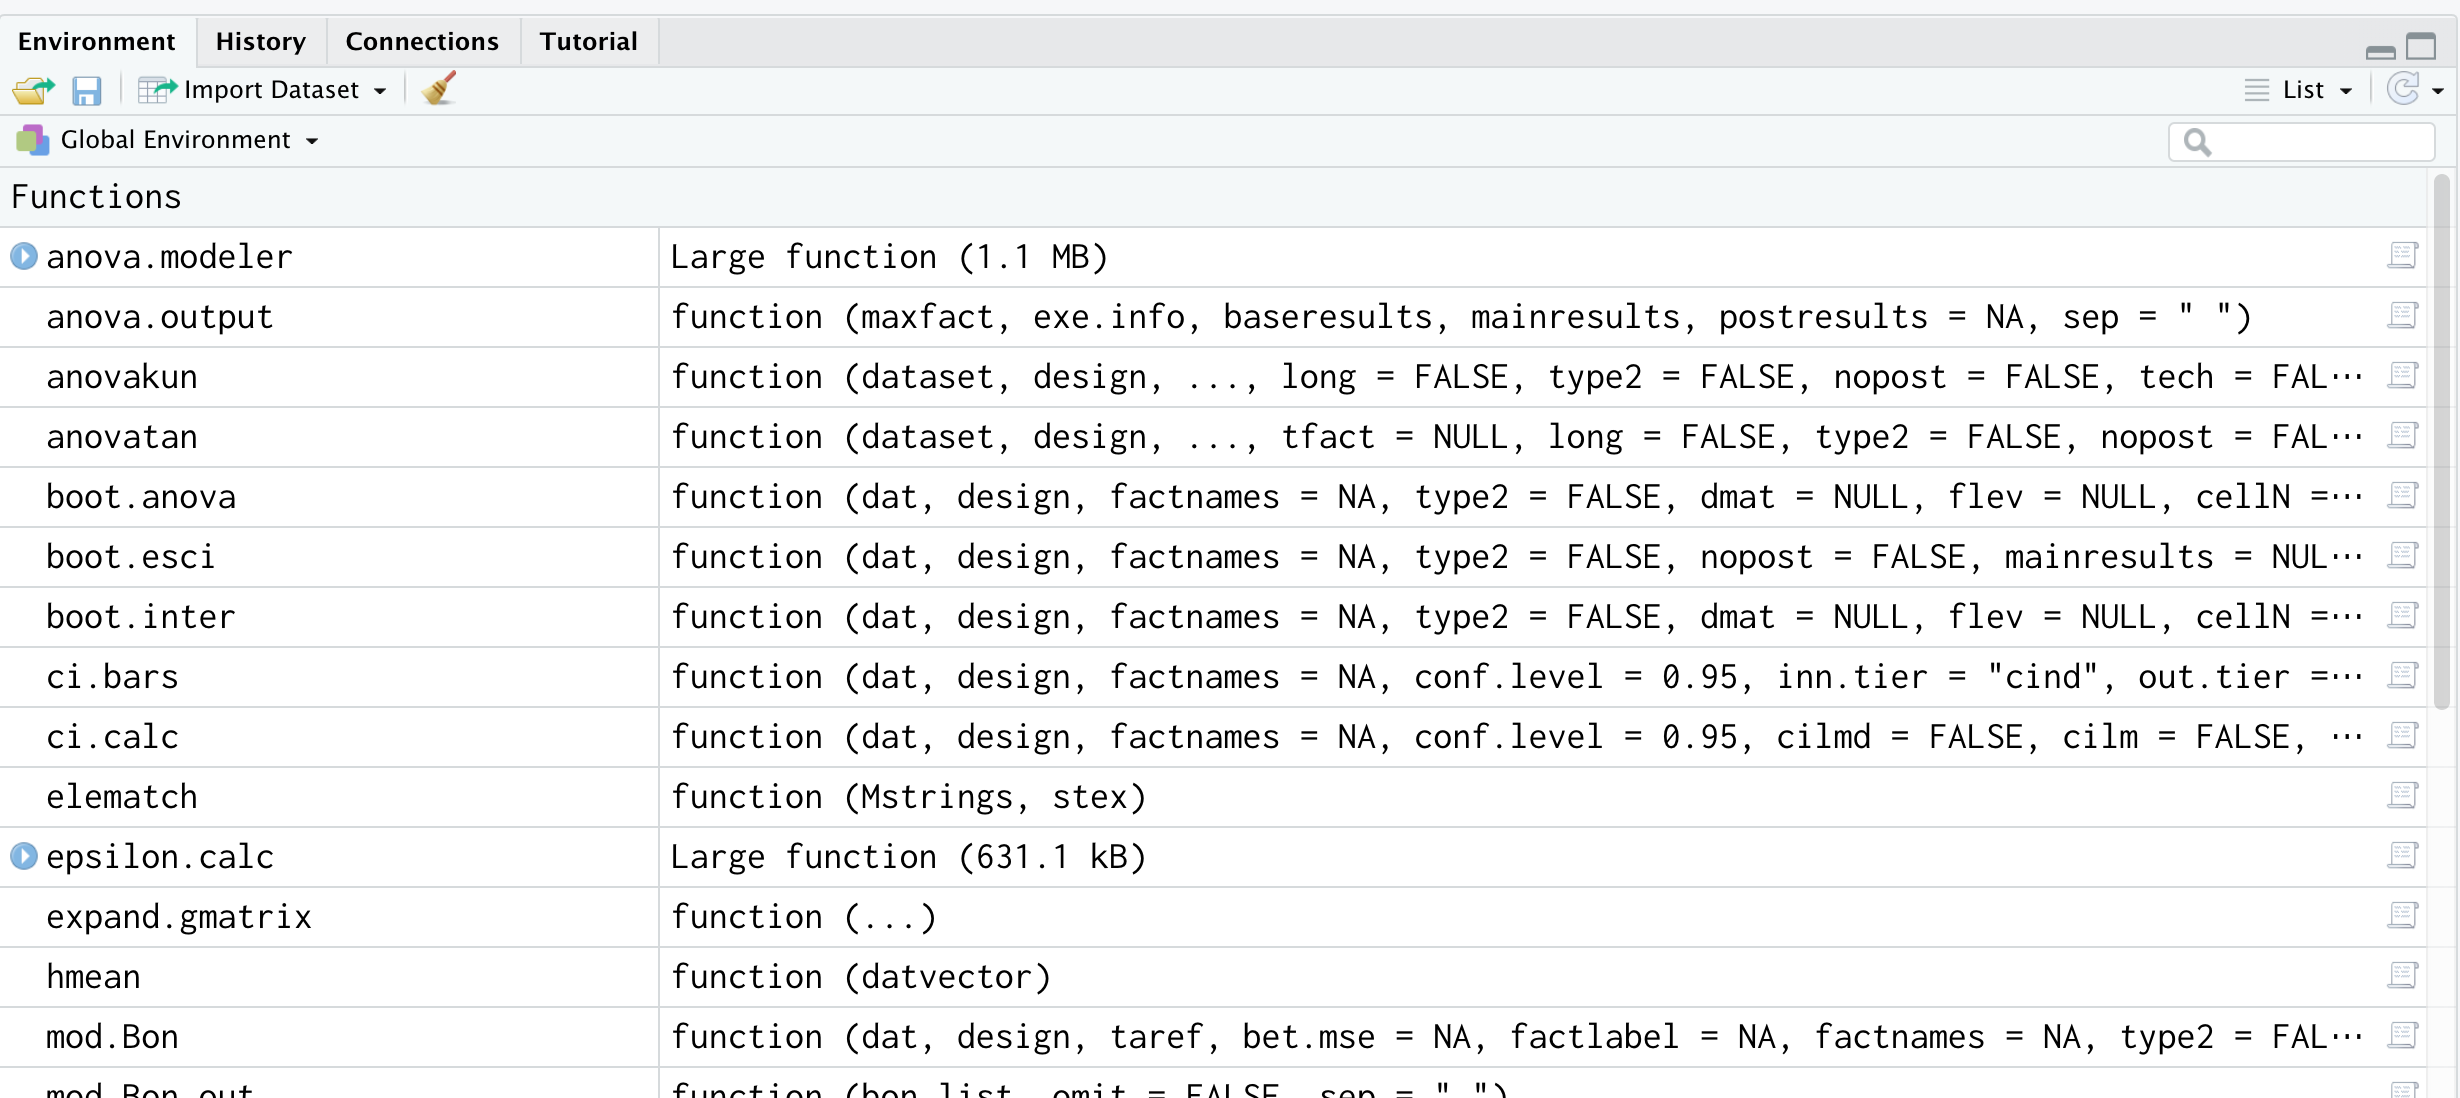
\includegraphics[keepaspectratio,width=0.8\linewidth]{figures/20_anovakun/anovaku_funcs.png}
	\caption{anovakunを読み込んだあとの環境タブ}
	\label{fig:20_01}
\end{figure}
それでは実際の使い方を見ていきましょう。

\section{データの作りかた}
\label{MakingData}
\subsection{よいデータの形式とは}
分析に先立って，データをどのように準備するかについて説明しておきます。
みなさんは既に心理学基礎実験などで，データを使って・作って集計したり分析したことがあるかもしれません。その際はデータの入力の仕方について，テキストや資料通りに進めたかもしれませんが，実際に自分で研究をするときは「どのようにデータを入力するか」も自分で考えることになります。このとき，分析しにくい形でデータを作ってしまうと，後で分析に苦労することになります。そこで，分散分析を行う際に適したデータの形について説明しておきます。

データが数件しかないのであれば，これまでのように手入力することになるでしょう。しかしデータが多くなってくると，入力するところだけは表計算ソフトを使う方が便利です\footnote{データを入力するために使い，その後の分析は全てRでやるのが得策です。表計算ソフトで平均や分散などの数値を特定のセルに計算してしまうと，それを読み込んでRで分析するときに邪魔になります。とったデータだけの生のデータ(ロウデータといいます)はRで読み込み可能なCSV形式などで保存し，以降の処理は全て記録の残るRでやるようにしましょう。}。このときに注意すべきことは，\textbf{1つのセルには1つのデータしか入れない}ということです。これからデータを色々加工していきますが，加工する前のデータはなるべくプレーンな状態であったほうが良いのです(すでに加工された食材を違う料理に利用するのは大変ですから！)。

例えば図\ref{fig:20_02}は，悪いデータファイル作成の例です。これをまずはじっくり眺めて，どこがまずいのか考えてみてください。少なくとも7つの点で問題があります。
\begin{center}
	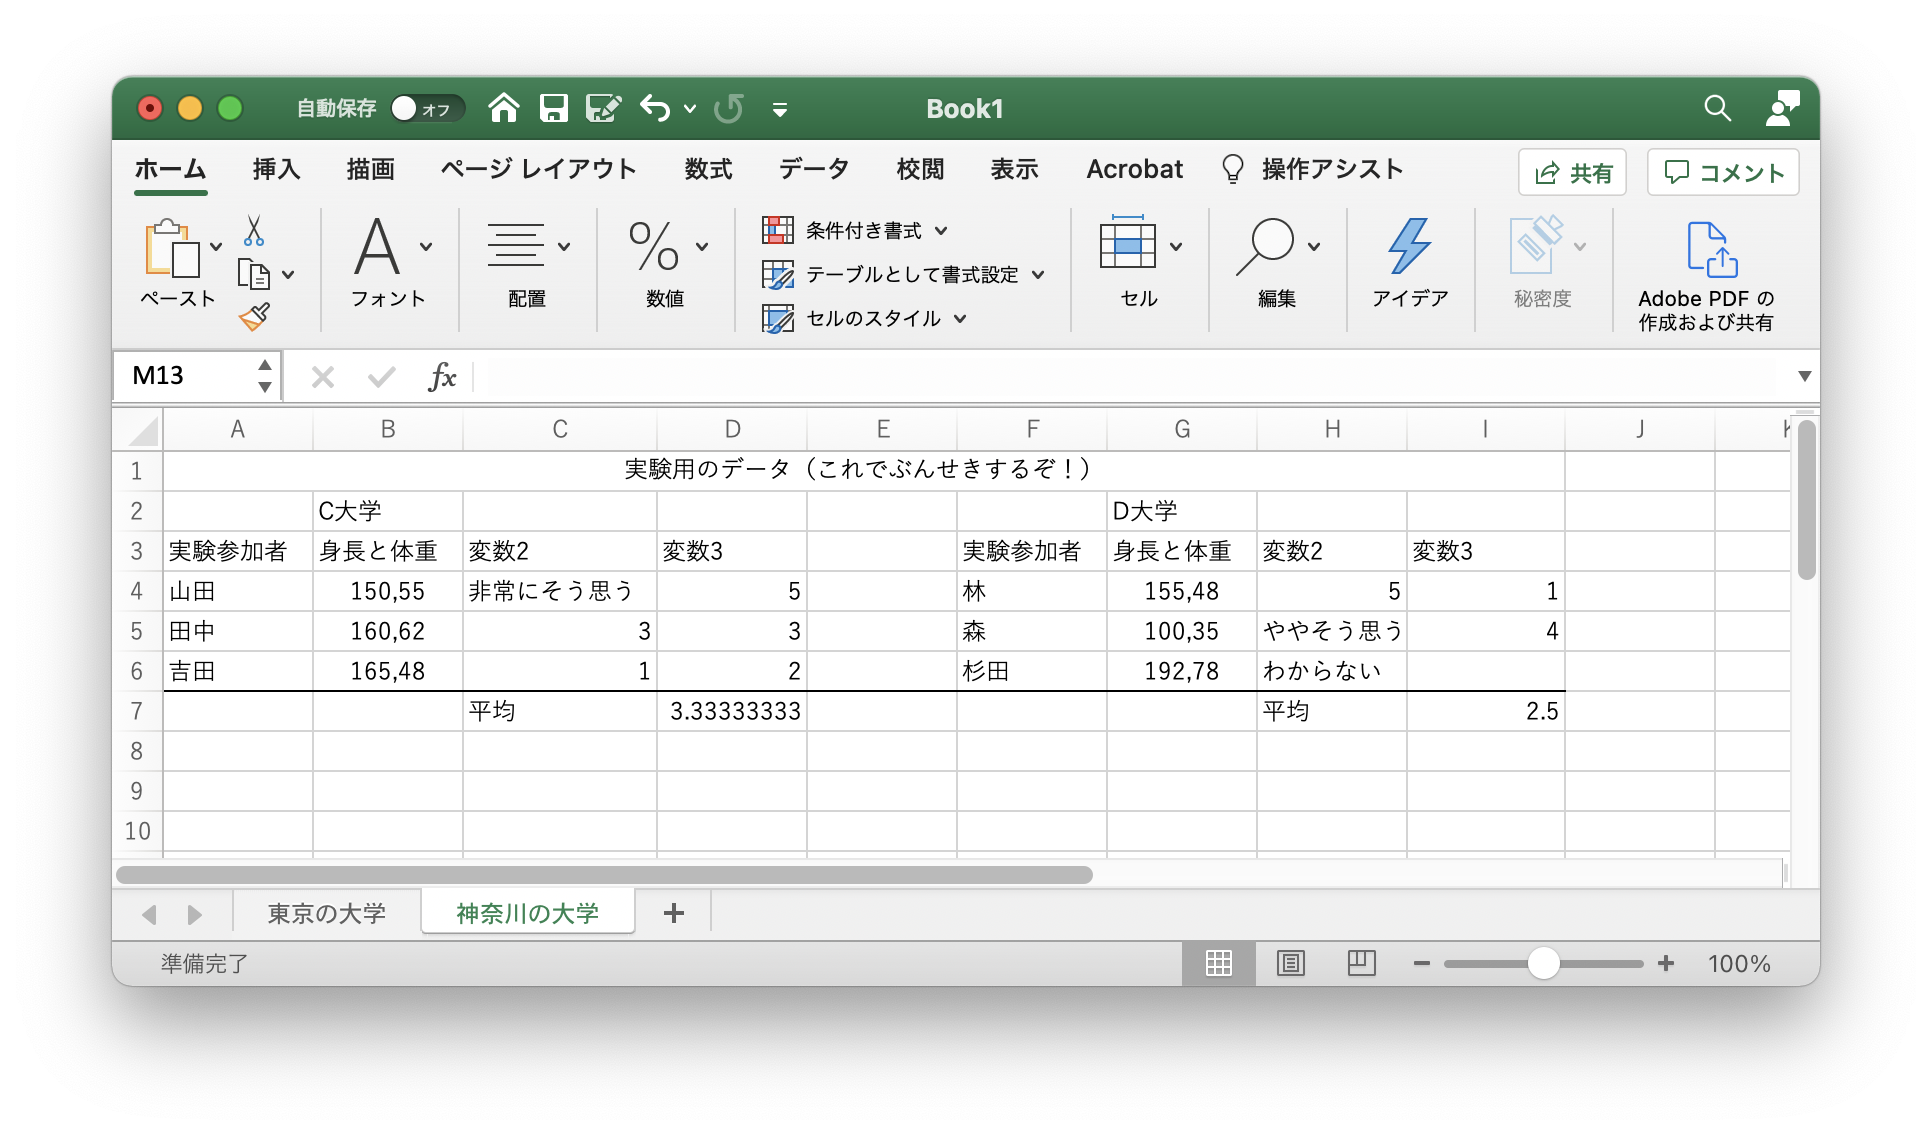
\includegraphics[keepaspectratio,width=\linewidth]{figures/20_anovakun/dataSheet.png}
	\captionof{figure}{分析に不向きなデータファイル}
	\label{fig:20_02}
\end{center}

分析しにくいよくないデータになっているのは次の箇所です。
\begin{enumerate}
	\item 1行目にこの表のタイトルのようなものが入っていますが，これは分析には使わない情報なので不要です。
	\item 1行目はセルを結合しています。データセットは\texttt{data.frame}型のように矩形であるべきなので，データのサイズを狂わせる行の存在は不適切です。
	\item 2行目には大学名が入っているようです。AからD列はC大学，FからIはD大学のデータのようですが，1つのデータセットに複数のデータが混在しているのはよくありません。
	\item 身長と体重，という変数名のところには1つのセルに複数の数字が入っています。カンマで区切られており，見た目にはわかりますが，機械的には(カンマのせいで)数字ではなく文字列として扱われます。データがデータになっていないのです。
	\item 変数2の列は「非常にそう思う」という言葉の回答と，数字が入っています。1つの列の中に複数の種類のデータが含まれるので分析できません(文字と数字の集計ができない。ちなみにこの場合は文字変数として扱われます)。
	\item 7行目に平均とありますが，データの平均はデータから計算できる量なので，Rで算出するものです。データの中に計算結果を入れておくべきではありません。
	\item I列6行目，D大学の杉田さんに関する変数3の箇所が空欄です。これはデータが入手できなかったところかもしれませんが，これは欠測値であることを明示すべきです。
	\item 「東京の大学」と「神奈川の大学」という複数のシートがあります。データファイルとしては1つのシートにすべての情報が入っていなければなりません。同時に分析できるデータなのであれば，一枚のシートにまとめるべきです。
\end{enumerate}
皆さんはいくつ気づいたでしょうか。これらの問題点を通じて言えることは「1つのデータセット，1つのセルには過不足ない情報を入れる」ということです。表を作って見せるのであればこのような入力でも良いのですが，ここでは数値データを分析することが目的なのですから，レイアウトや数字でない情報，計算してここから作れる情報は，分析に必要のない過剰な情報なのです。ちなみにアンダーラインや文字色，セルの色などは分析の時に自動的に受け落ちます(データではない情報なので)。表計算ソフトは数字を表にして計算するソフトウェアであり，方眼用紙やレイアウトする文書とは異なることを意識しましょう。

加えて分析の時に不便なのは，文字と数字の関係です。1つのセルに複数の数字が入る場合，区切り記号などをつけることが多いかと思いますが(スペースも機械にとっては文字です！)，こうした文字種・変数の種類・水準が混在しているのも情報過多ということになります。

今回の問題点を修正したのが図\ref{fig:20_03}のようなデータセットです。単一のデータセットで完結しています。また1つの列に一種類の変数，不要な情報はなく，過剰な情報もないデータセットになっているのがわかるかと思います。なお，変数3のところに\texttt{NA}とあるのは\texttt{No Answer}の略で\keyterm{欠測値}{けっそくち}{missing value}を意味しています。これは読み込む時に，欠測値をどのような文字にしているか，という指定ができますので問題になりません。
\begin{center}
	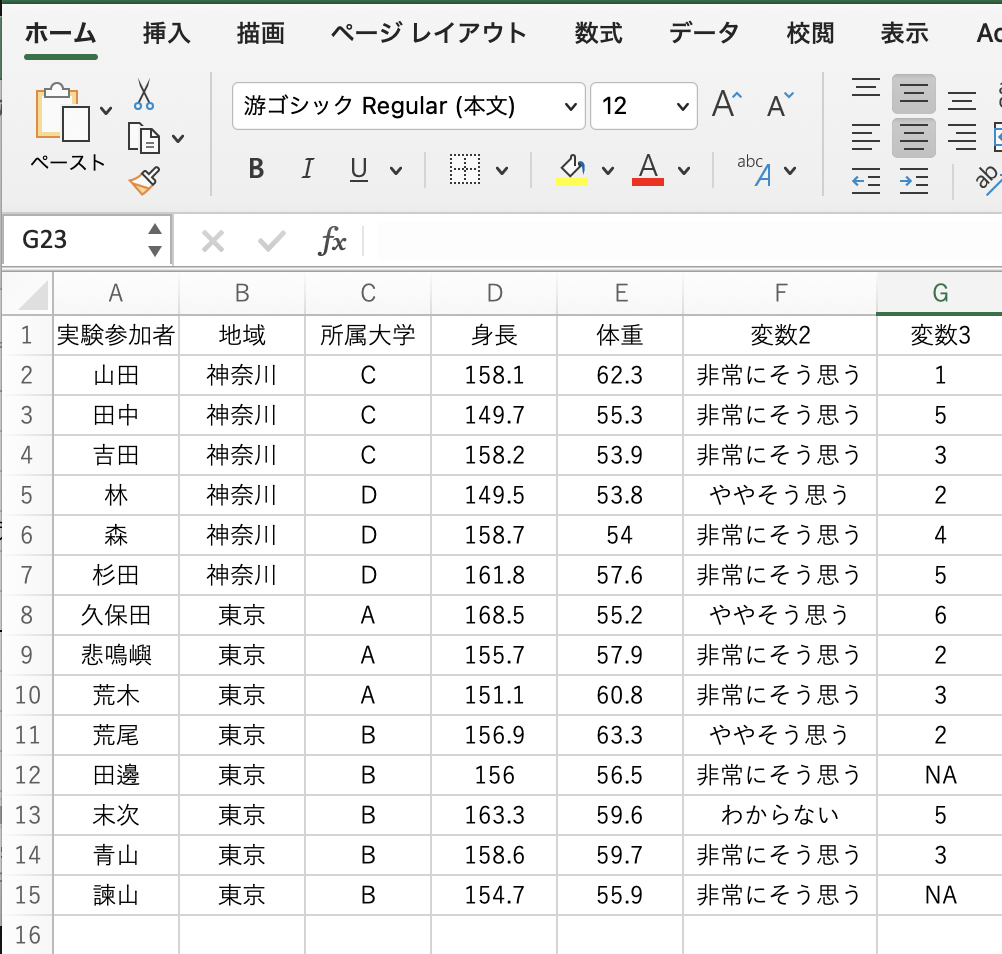
\includegraphics[keepaspectratio,width=0.8\linewidth]{figures/20_anovakun/dataSheet2.png}
	\captionof{figure}{分析に適したデータファイル}
	\label{fig:20_03}
\end{center}

このように，データの入力の基本は，\textbf{1行に1ケースの情報が入っている，過不足のない1つのデータセットを作ること}である，と言えます。

このようにして作られたデータファイルは，UTF-8の文字コードによるcsv形式で保存するのが基本です($\to$付録\ref{computer}，\ref{suffix}節，Pp.\pageref{suffix}参照)。ファイルを保存する時に，ファイル形式をしっかり指定し，拡張子も\texttt{.csv}にしましょう。csvファイルはASCIIファイルですし，文字コードも世界基準のUTF-8にしておけばどのPCからでもみることができます。ある一企業が開発した特定のOS，特定のアプリケーションを持っていなければデータを見ることができない，というのは科学的研究の観点からは不適切なのです。

ちなみに2020年12月，総務省により機械判読可能なデータの表記方法の統一ルールが策定されました\parencite{soumu}。それには次のようなチェック項目が含まれています。
\begin{description}
	\item[チェック項目1-1] ファイル形式はExcelかCSVとなっているか
	\item[チェック項目1-2] 1セル1データとなっているか
	\item[チェック項目1-3] 数値データは数値属性とし，文字列を含まないこと
	\item[チェック項目1-4] セルの結合をしていないか
	\item[チェック項目1-5] スペースや改行等で体裁を整えていないか
	\item[チェック項目1-6] 項目名を省略していないか
	\item[チェック項目1-7] 数式を使用している場合は，数値データに修正しているか
	\item[チェック項目1-8] オブジェクトを使用していないか
	\item[チェック項目1-9] データの単位を記載しているか
	\item[チェック項目1-10] 機種依存文字を使用していないか
	\item[チェック項目2-1] データが分断されていないか
	\item[チェック項目2-2] 1シートに複数の表が掲載されていないか
\end{description}
みなさんも自分でデータを作るときは，こうした基準に沿うように心がけてください。
また表計算ソフトの中で，代表値を計算したりグラフを書いたりしたくなりますが，みなさんは既に統計環境を手に入れているのですから，そうした加工・可視化などはRのほうでやり，データは「誰が触っても良いプレーンな素材」として保管しておくように心がけましょう。

\subsection{整然データ}
データ入力の時に見たように，データファイルは1セルに1情報，重複や集計，オブジェクトや文字列のないデータセットであることが基本です。
また図\ref{fig:20_03}にあるように，一行ごとに1人(1ケース，1オブザベーション，1レコードとも言います)のデータが入っており，各列が変数を表していることが一般的です。変数が増えると横に伸びていきますので，こうしたデータの入力形式を\keytermL{ワイド型}{わいどがた}のデータということがあります。

ここで表\ref{tbl:20_01}を見てください。このデータを見ると我々は，「大阪の午後は曇りなんだな」ということがすぐにわかります。
\begin{center}
	\captionof{table}{ワイド型データ}
	\begin{tabular}{c|cccc}
		   & 午前 & 午後 & 夕方 & 深夜 \\\hline
		東京 & 晴  & 晴  & 雨  & 雨  \\
		大阪 & 晴  & 曇  & 晴  & 晴  \\
		福岡 & 晴  & 曇  & 曇  & 雨  \\\hline
	\end{tabular}
	\label{tbl:20_01}
\end{center}
しかしその判断は，「大阪」行の「午後」列を見て，すなわち行と列に素早く目を走らせてそれのクロスするところで「曇」という情報を得ています。夕方や深夜の情報が知りたければ，列を変えますね。列ごとに違う変数になっているから当然です。行と列の名前を参照するというのは，目線を左右と上下に動かす2アクション必要なことです。

しかしここで参照している「列名(変数名)」も変数，データの一部ではないでしょうか。この観点に立ち，1行見るだけですべての情報がわかるようにしてみましょう。表\ref{tbl:20_02}には表\ref{tbl:20_01}と同じ情報しか含まれていませんが，一行見るだけですべての情報がわかるようになっています。

\begin{center}
	\captionof{table}{ロング型データ}
	\begin{tabular}{ccc}
		地域 & 時間帯 & 天候 \\\hline
		東京 & 午前  & 晴  \\
		東京 & 午後  & 晴  \\
		東京 & 夕方  & 雨  \\
		東京 & 深夜  & 雨  \\
		大阪 & 午前  & 晴  \\
		大阪 & 午後  & 曇  \\
		大阪 & 夕方  & 晴  \\
		大阪 & 深夜  & 晴  \\
		福岡 & 午前  & 晴  \\
		福岡 & 午後  & 曇  \\
		福岡 & 夕方  & 曇  \\
		福岡 & 深夜  & 雨  \\\hline
	\end{tabular}
	\label{tbl:20_02}
\end{center}

表\ref{tbl:20_02}のような形のデータのことを，\keytermL{ロング型}{ろんぐがた}のデータと言います。
このような形にしておくと，情報の欠落(欠測値)があった時の対応が楽に行えたり，レコードの選択がやりやすくなるなどの利点があります。

このような分析しやすいデータの形について，\textcite{Hadley2014}が提唱したのが\keyterm{整然データ}{せいぜんでーた}{Tidy Data}という考え方です。整然データとは，次の4つの特徴を持ったデータ形式のことです。
\begin{itemize}
	\item 個々の変数(variable)が1つの列(column)をなす。
	\item 個々の観測(observation)が1つの行(row)をなす。
	\item 個々の観測の構成単位の類型(type of observational unit)が1つの表 (table) をなす。
	\item 個々の値 (value) が1つのセル (cell) をなす。
\end{itemize}
さきほどの天気の例では，時間，場所，天候という3つの情報が表に含まれていますが，これが一行の中にまとまっているのが整然データです。
人間にとってはワイド型のデータの方がわかりやすいこともありますが，分析を進めていく上ではロング型・整然データの方が便利なことも多くあります。たとえばこの後で行う作図においては，整然データの方が便利な形です。X軸に割り当てる列，Y軸に割り当てる列，色や形を指定する列，など列ごとに持つ特徴を図の設定に割り当てることができるからです。

実際にデータを入力するときは，人間にとってわかりやすいワイド型が便利ですが，統計的な処理をしたり，グラフを描画するときにはロング型の整然データの方が便利です。そこで，ワイド型のデータをロング型の整然データに変換する方法を学びましょう。ありがたいことに，\verb|tidyverse|というパッケージを用いると，こうしたデータの加工が非常に楽に行える関数をいろいろ使うことができます。

\subsection{分散分析のデータ形式}

では実際に分散分析を行う際は，どのようなデータ形式にすればよいのでしょうか。\verb|anovakun|はロング型にもワイド型にも対応していますが，まずはワイド型で入力する方がわかりやすいでしょう。すなわち，各列が変数を表し，各行が1人(1ケース)のデータを表す形です。

群内要因のデータを列(横)に並べ，群間要因のデータを行(縦)に並べるのが基本です。次の例は，2要因の混合計画(間(3)$\times$内(2))のデータ例です。

\begin{lstlisting}[language=c++,label={code:20_03},caption={データの準備}]
rm(list=ls())
library(tidyverse)
MixedDesign <- data.frame(id = 1:12,
                       condition = rep(1:3,each=4),
                       stimuli1 = c(6,6,5,5,7,4,7,6,4,3,4,6),
                       stimuli2 = c(8,3,2,5,9,7,1,6,4,9,2,3))
# 要因型にする
MixedDesign$condition <- factor(MixedDesign$condition,
                             labels = c("control","exp1","exp2"))
print(MixedDesign)
\end{lstlisting}
\paragraph{コード解説}
\begin{description}
	\item[1行目] 作業スペースをクリアしています。
    \item[2行目] \verb|tidyverse|パッケージを読み込んでいます。
    \item[3-7行目] データフレームを作成しています。被験者ID，条件変数，刺激1，刺激2の4つの変数があります。
    \item[8-10行目] 条件変数を要因型にしています。ラベルは統制群(control)と実験群1(exp1)，実験群2(exp2)としています。
    \item[11行目] データフレームを表示させています。
\end{description}

\begin{Rscreen}{ワイド型データの出力}{out20_01}
\begin{verbatim}
   id condition stimuli1 stimuli2
1   1   control        6        8
2   2   control        6        3
3   3   control        5        2
4   4   control        5        5
5   5      exp1        7        9
6   6      exp1        4        7
7   7      exp1        7        1
8   8      exp1        6        6
9   9      exp2        4        4
10  10     exp2        3        9
11  11     exp2        4        2
12  12     exp2        6        3
\end{verbatim}
\end{Rscreen}
どこに何が入っているか，どのようにデータフレームを汲み上げているかを確認してください。

さてここで，\verb|tidyverse|パッケージを使うとワイド型とロング型を相互に変換できることを説明しておきます。ワイド型のデータをロング型に変換するには，\verb|pivot_longer()|関数を使います(\texttt{code:\ref{code:20_04}})。

\begin{lstlisting}[language=c++,label={code:20_04},caption={ワイド型からロング型への変換}]
MixedDesign_long <- MixedDesign %>%
  pivot_longer(cols = c(stimuli1,stimuli2),
               names_to = "stimuli",
               values_to = "value")
print(MixedDesign_long)
\end{lstlisting}

\paragraph{コード解説}
\begin{description}
    \item[1行目] ワイド型のデータフレームをロング型に変換し，新しいデータフレーム\texttt{MixedDesign\_long}に代入しています。
    \item[2-4行目] \verb|pivot_longer()|関数を使って，\texttt{stimuli1}と\texttt{stimuli2}の列をロング型に変換しています。変換後の変数名は\texttt{stimuli}，値の入る変数名は\texttt{value}としています。
    \item[5行目] 変換後のデータフレームを表示させています。
\end{description}

\begin{Rscreen}{ロング型データの出力}{out20_02}
\begin{verbatim}
> print(MixedDesign_long)
# A tibble: 24 × 4
      id condition stimuli  value
   <int> <fct>     <chr>    <dbl>
 1     1 control   stimuli1     6
 2     1 control   stimuli2     8
 3     2 control   stimuli1     6
 4     2 control   stimuli2     3
 5     3 control   stimuli1     5
 6     3 control   stimuli2     2
 7     4 control   stimuli1     5
 8     4 control   stimuli2     5
 9     1 exp1      stimuli1     7
10     1 exp1      stimuli2     9
# ℹ 14 more rows
# ℹ Use `print(n = ...)` to see more rows
\end{verbatim}
\end{Rscreen}
どのようにデータフレームが変わったか，よく確認してください。ロング型データにしておくと，後でグラフを描くときに便利です。

\section{二要因Between計画の実際}
それでは実際に\verb|anovakun|を使って，二要因計画の分散分析を実行してみましょう。データは第\ref{ch18_BetweenDesign}章で使ったものと同じです(再掲。表\ref{tbl:20_03})。コーヒーの温度(Hot vs Cold)とメーカー(銘柄A vs 銘柄B)の2要因があり，それぞれの条件で3人ずつ被験者がいて，コーヒーの味の評価を行った，というデータです。

% latex table generated in R 4.0.2 by xtable 1.8-4 package
% Fri Sep 11 14:11:29 2020
\begin{table}[ht]
	\centering
	\caption{二要因のデータ例}
	\begin{tabular}{rrllr}
		\hline
		通し番号 & 群での番号 & 温度   & メーカー & 評価 \\
		\hline
		1    & 1     & Hot  & 銘柄A  & 13 \\
		2    & 2     & Hot  & 銘柄A  & 11 \\
		3    & 3     & Hot  & 銘柄A  & 12 \\
		4    & 1     & Hot  & 銘柄B  & 7  \\
		5    & 2     & Hot  & 銘柄B  & 6  \\
		6    & 3     & Hot  & 銘柄B  & 8  \\
		7    & 1     & Cold & 銘柄A  & 9  \\
		8    & 2     & Cold & 銘柄A  & 9  \\
		9    & 3     & Cold & 銘柄A  & 9  \\
		10   & 1     & Cold & 銘柄B  & 13 \\
		11   & 2     & Cold & 銘柄B  & 11 \\
		12   & 3     & Cold & 銘柄B  & 9  \\
		\hline
	\end{tabular}

	\label{tbl:20_03}
\end{table}
これをデータフレーム型にします。温度，メーカーは名義尺度水準なので要因型にします(\texttt{code:\ref{code:20_05}})。ID変数は特に必要ありませんので，省略しています。
\begin{lstlisting}[language=c++,label={code:20_05},caption={データフレームにする}]
Between2 <- data.frame(
  temp = rep(1:2, each = 6),
  maker = rep(rep(1:2, each = 3), 2),
  value = c(13, 11, 12, 7, 6, 8, 9, 9, 9, 13, 11, 9)
)
Between2$temp <- factor(Between2$temp,labels = c("Hot", "Cold"))
Between2$maker <- factor(Between2$maker,labels = c("A", "B"))
\end{lstlisting}


ではこれを\texttt{anovakun}でやってみましょう。彼(?)なら一気にすべての答えを出してくれるのです(\texttt{code:\ref{code:20_06}})。
\begin{lstlisting}[language=c++,label={code:20_06},caption={anovakunで実行}]
anovakun(Between2,"ABs",2,2,eps = T)
\end{lstlisting}

\verb|anovakun|関数の使い方のポイントは，要因計画の型を文字列で指定するところです。詳しくは開発者である井関先生のサイト\footnote{\url{https://riseki.cloudfree.jp/?ANOVA君/ANOVA君の使い方}}を参照してもらいたいのですが，基本的な使い方は次の通りです。

\verb|anovakun(データ, "要因計画の型", 各要因の水準数，...)|

ここで「要因の型」を指定する部分ですが，2要因間$\times$間計画の場合は\texttt{ABs}とします。小文字のsは実験参加者を表していて，sの左側にあるのは群間要因，sの右側にあるのは群内要因を表しています。要因にはA,B,C,...,Z でラベルをつけます。今回のように間$\times$間の場合は，\texttt{ABs}となります。内$\times$内の場合は\texttt{sAB}，混合計画の場合は\texttt{AsB}や\texttt{BsA}などとします。最後の\texttt{eps=T}は，効果量である$\varepsilon^2$を表示するスイッチをオン(TRUE)，ということです。

結果は\texttt{Rの出力\ref{RS:out20_03}}のように表示されます。
\begin{Rscreen}{ABsタイプの出力}{out20_03}
	\begin{verbatim}
[ ABs-Type Design ]

This output was generated by anovakun 4.8.9 under R version 4.5.1.
It was executed on Sun Oct 19 15:45:02 2025.

 
<< DESCRIPTIVE STATISTICS >>

-------------------------------
  A   B   n     Mean    S.D. 
-------------------------------
 a1  b1   3  12.0000  1.0000 
 a1  b2   3   7.0000  1.0000 
 a2  b1   3   9.0000  0.0000 
 a2  b2   3  11.0000  2.0000 
-------------------------------


<< ANOVA TABLE >>

---------------------------------------------------------------
 Source      SS  df      MS  F-ratio  p-value      epsilon^2 
---------------------------------------------------------------
      A  0.7500   1  0.7500   0.5000   0.4996 ns     -0.0133 
      B  6.7500   1  6.7500   4.5000   0.0667 +       0.0933 
  A x B 36.7500   1 36.7500  24.5000   0.0011 **      0.6267 
  Error 12.0000   8  1.5000                                  
---------------------------------------------------------------
  Total 56.2500  11  5.1136                                  
                   +p < .10, *p < .05, **p < .01, ***p < .001


<< POST ANALYSES >>

< SIMPLE EFFECTS for "A x B" INTERACTION >

---------------------------------------------------------------
 Source      SS  df      MS  F-ratio  p-value      epsilon^2 
---------------------------------------------------------------
A at b1 13.5000   1 13.5000   9.0000   0.0171 *       0.2133 
A at b2 24.0000   1 24.0000  16.0000   0.0039 **      0.4000 
B at a1 37.5000   1 37.5000  25.0000   0.0011 **      0.6400 
B at a2  6.0000   1  6.0000   4.0000   0.0805 +       0.0800 
  Error 12.0000   8  1.5000                                  
---------------------------------------------------------------
                   +p < .10, *p < .05, **p < .01, ***p < .001

output is over --------------------///
\end{verbatim}
\end{Rscreen}


最初に，水準ごとの平均値と標準偏差が表示され，続いて分散分析表が示されています。ご丁寧に有意かどうかわかりやすいような記号(\verb|.|や\verb|*|など)がついています。最後の一行には\texttt{+p < .10, *p < .05, **p < .01, ***p < .001}とありますが，これは米印が1つなら5\%，2つなら1\%，3つなら0.1\%水準で有意である，という意味です。さらに，\verb|+|の記号であれば10\%水準で有意であるということもわかります\footnote{おそらくこれが諸悪の根源で，なんとなく星の数が多い方が「良い結果」のような印象を持ちますし，分析したらとりあえず星を探す，という仕草が生まれるようになっていますよね。帰無仮説検定はあくまでもモデル比較の判定であって，判定基準が厳しいほど「良い」とか，基準をクリアできなかったから「惜しい(残念)」という評価を伴うものではないはずなのに，です。有意差がなかったら，そういう結果が得られた，というだけですし，星の数が小さくてもえらいとかすごい，ということにはならない，ということを再確認してください。「心理学者は星を探して喜んでるんだ」というようなジョークの的にならないように，適切な分析的素養を身に付けましょう。}。これを見ると，要因A(温度)の主効果はなく($F(1,8)=0.500,p=0.4996$)\footnote{米印があるべきところに$ns$とありますが，これはnot significant，つまり有意ではないという意味です。}，ついで要因Bの効果も5\%水準では認められない(10\%水準で有意，その記号として$+$が使われています)\footnote{世の中には「有意傾向」という変な言葉があります。今回要因Bの$p$値は6\%でしたが，これは5\%水準ではアウトですよね。こういった5\%をちょっとだけ上回っちゃった，惜しい！という時に，「有意になりそうな傾向があった」略して「有意傾向があった」という表現がされることがあるのです。あるいは「傾向差があった」という言葉もまことしやかに使われていたりします。が，これらは心理学独自の間違った表現であり，決して使うべきではありません。なぜなら，5\%だろうが6\%だろうが，任意に決めた判定基準であって，$p$ 値の大小関係は現実の効果の大きさとは関係がないからです。}，また交互作用は5\%水準で有意という結果になりました。さらに効果量$\varepsilon^2$の列を見ると，交互作用は全体の62\%の分散を説明したことになりますから，これはかなり大きな効果だったようだ，ということがわかります。

続いてPOST ANALYSISとして事後の検定が表示されています。SIMPLE EFFECTS for "A x B" INTERACTIONとあるのは，「AとBの交互作用についての単純効果」という意味で(直訳！)，各水準に限定した時に他の水準の効果があったかどうかをみています。たとえば最初の行，A at b1とありますが，これは要因B(銘柄)の第一水準における要因A(温度)の効果をみていることになります。以下同様ですが，これらは分散分析の表をより細かくしてチェックしているようなものです。これを見ると，冷たい時の銘柄には差がない(B at a2)ようですが，それ以外の差は統計的に有意，と言えそうです。

これらの結果を報告する時は，次のように書くと良いでしょう。
\begin{quote}
	温度と銘柄の効果を独立変数とした二要因分散分析($2 \times 2$のBetweenデザイン)をおこなったところ，交互作用が有意($F(1,8)=24.5,p=0.0011,\varepsilon^2=0.6267$)になり，事後の検定の結果，銘柄Aにおける温度の効果($F(1,8)=9.0,p=0.0171,\varepsilon^2=0.2133$)，銘柄Bにおける温度の効果($F(1,8)=16.0,p=0.0039,\varepsilon^2=0.4000$)，および温かい時の銘柄の効果($F(1,8)=25.0,p=0.0011,\varepsilon^2=0.6400$)が統計的に有意であった。
\end{quote}

これらの結果を見やすくするために，図\ref{fig:20_04}に可視化してみました。
\begin{figure}[ht]
	\centering
	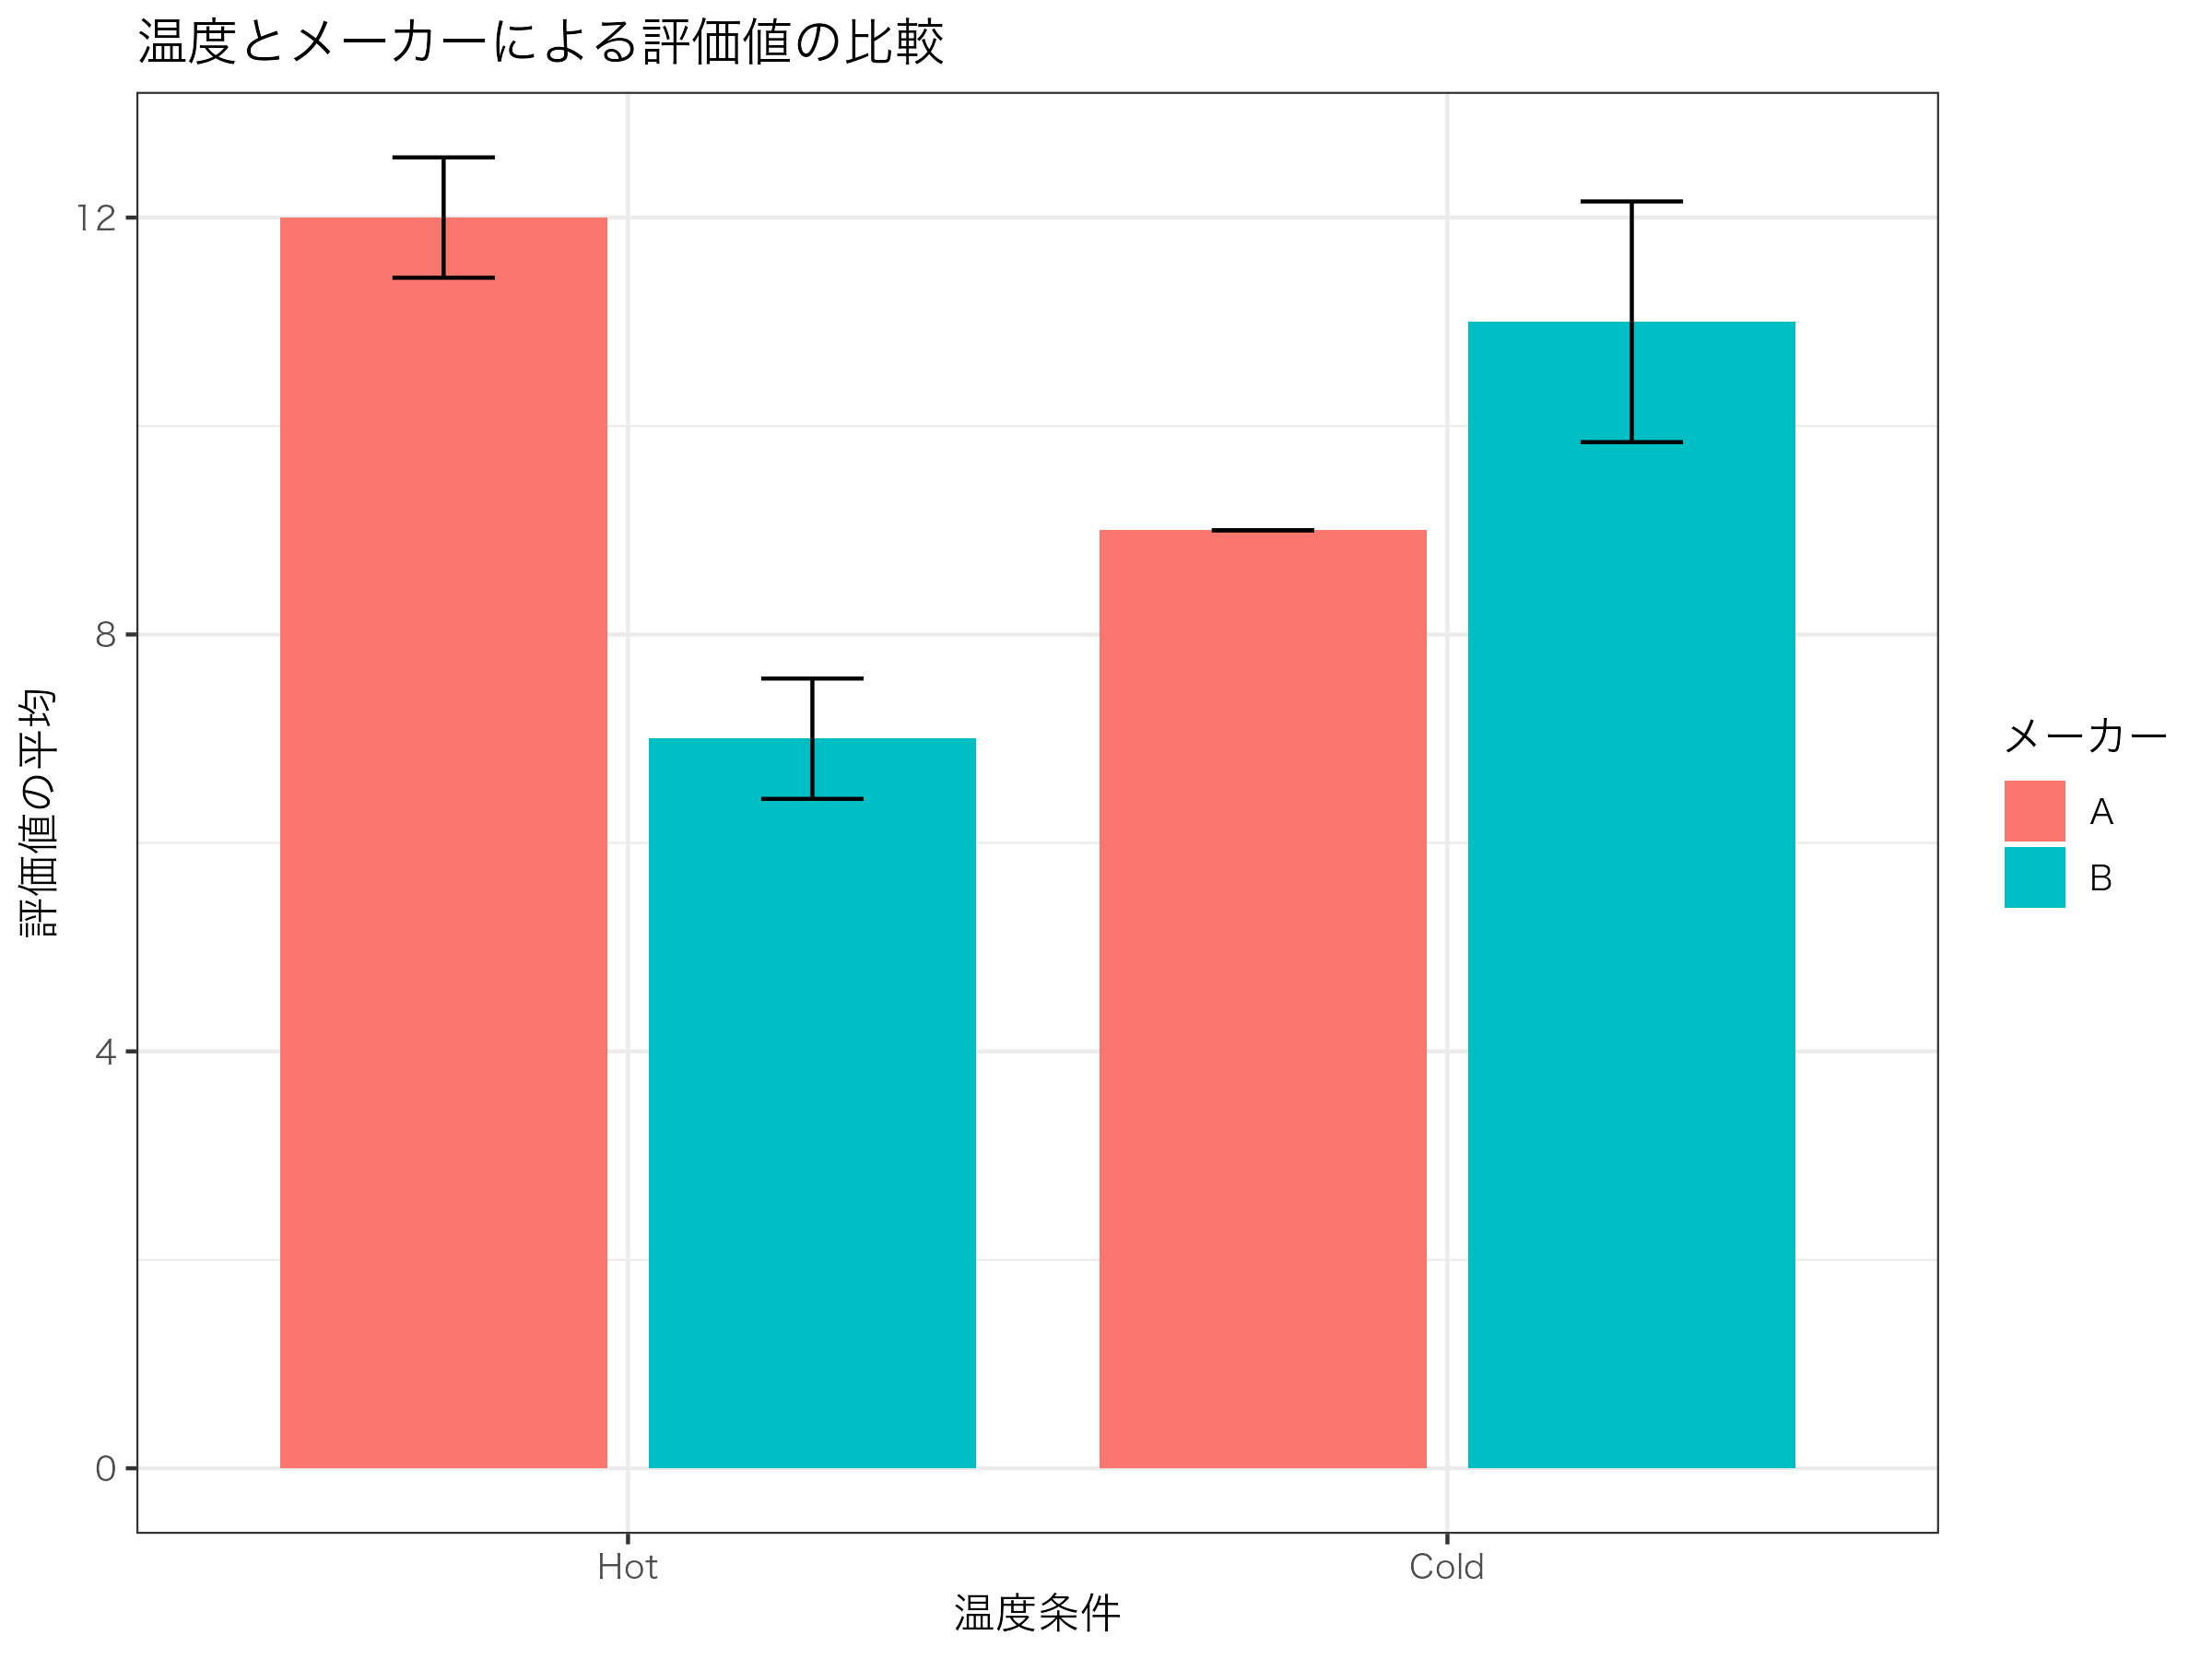
\includegraphics[keepaspectratio,width=0.8\linewidth]{figures/20_anovakun/anova_figures.png}
	\caption{POST ANALYSISの検定結果の確認}
	\label{fig:20_04}
\end{figure}

この図を書いたのは次のコードによるものです。コードの書き方は参考程度で結構ですが\footnote{このコードは生成AIのひとつ，Claude(Sonnet4.5モデル)に「Between2をつかった分散分析の結果をggplot2で可視化するコードをかけ」と指示して書かせたものです。このように生成AIを使うとRのコードも書いてくれますのでコード自体を恐れる必要はありません。人間に必要なのは適切な指示を出すこと，ゴールのビジョンを明確に持つことです。}，どのようにして可視化できるかを確認してください(\texttt{code:\ref{code:20_07}})。
\begin{lstlisting}[language=c++,label={code:20_07},caption={可視化のコード}]
Between2 %>%
  group_by(temp, maker) %>%
  summarise(
    mean = mean(value),
    sd = sd(value),
    n = n(),
    se = sd / sqrt(n),
    .groups = "drop"
  ) %>%
  ggplot(aes(x = temp, y = mean, fill = maker)) +
  geom_bar(
    stat = "identity",
    position = position_dodge(0.9),
    width = 0.8
  ) +
  geom_errorbar(aes(ymin = mean - se, ymax = mean + se),
    position = position_dodge(0.9), width = 0.25
  ) +
  labs(
    title = "温度とメーカーによる評価値の比較",
    x = "温度条件",
    y = "評価値の平均",
    fill = "メーカー"
  ) +
  theme_bw()
\end{lstlisting}
\paragraph{コード解説}
\begin{description}
    \item[1行目] データフレーム\texttt{Between2}をパイプでつないでいます。
    \item[2行目] \verb|group_by()|関数で，温度(\texttt{temp})とメーカー(\texttt{maker})の組み合わせごとにグループ化しています。
    \item[3-7行目] \verb|summarise()|関数で各グループの記述統計量を計算しています。平均値(\texttt{mean})，標準偏差(\texttt{sd})，サンプル数(\texttt{n})，標準誤差(\texttt{se})を算出し，\texttt{.groups = "drop"}でグループ化を解除しています。
    \item[8行目] パイプで\verb|ggplot()|関数に接続し，\texttt{aes()}で見た目の設定をしています。x軸に温度，y軸に平均値，塗りつぶしの色にメーカーを割り当てています。
    \item[9-12行目] \verb|geom_bar()|で棒グラフを描画しています。\texttt{stat = "identity"}で値をそのまま使い，\texttt{position\_dodge(0.9)}で棒を横に並べ，\texttt{width = 0.8}で棒の幅を指定しています。
    \item[13-15行目] \verb|geom_errorbar()|でエラーバー(標準誤差)を追加しています。\texttt{ymin}と\texttt{ymax}で誤差範囲を指定し，\texttt{position\_dodge(0.9)}で棒と位置を合わせ，\texttt{width = 0.25}でエラーバーの横幅を指定しています。
    \item[16-21行目] \verb|labs()|関数で図のタイトルと軸ラベルを設定しています。
    \item[22行目] \verb|theme_bw()|で白黒ベースのテーマを適用し，見やすいグラフにしています。
\end{description}

\newpage
\section{補遺；線形モデルとして分析}
ここまで\texttt{anovakun}パッケージを使って分散分析を行ってきましたが，Rの基本機能である線形モデルとしても同じ分析ができます。線形モデルで表現するには，次のようにします(\texttt{code:\ref{code:20_08}})。
\begin{lstlisting}[language=c++,label={code:20_08},caption={線形モデルとして実行}]
result.lm <- lm(value ~ temp * maker, data = Between2)
summary(result.lm)
\end{lstlisting}
ここで，説明変数が$\ast$でつなげられています。これで主効果と交互作用の両方をモデルの中に入れたことになります。結果は\texttt{Rの出力\ref{RS:out20_04}}のように表示されるはずです。

\begin{Rscreen}{交互作用を入れたモデルの出力}{out20_04}
	\begin{verbatim}
 > summary(result.lm2)

Call:
lm(formula = value ~ temp * maker, data = Example2)
 
Residuals:
    Min     1Q Median     3Q    Max 
-2.00  -0.25   0.00   0.25   2.00 

Coefficients:
                Estimate Std. Error t value Pr(>|t|)    
(Intercept)      12.0000     0.7071   16.97 1.48e-07 ***
tempCold         -3.0000     1.0000   -3.00  0.01707 *  
makerB           -5.0000     1.0000   -5.00  0.00105 ** 
tempCold:makerB   7.0000     1.4142    4.95  0.00112 ** 
---
Signif. codes:  0 ‘***’ 0.001 ‘**’ 0.01 ‘*’ 0.05 ‘.’ 0.1 ‘ ’ 1

Residual standard error: 1.225 on 8 degrees of freedom
Multiple R-squared:  0.7867,	Adjusted R-squared:  0.7067 
F-statistic: 9.833 on 3 and 8 DF,  p-value: 0.004641
\end{verbatim}
\end{Rscreen}

ここに示されているのは，温度\texttt{temp}変数の第一水準(Hot)かつメーカー\texttt{maker}変数の第一水準(銘柄A)を基準にした時に，\texttt{tempCold}つまりメーカーは同じ(銘柄A)で温度だけ違う群は平均値が$-3.0$，次にメーカーをBで\texttt{makerB}温度はHotの群と比べるとその平均値は$-5.0$，両方変えると$+7.0$になる，ということです。それぞれ標準誤差や$t$値が出ていますが，これは傾きが0である，という帰無仮説を棄却しているだけであって，効果の大きさについてはわかりません。

また，最後に$F$統計量が出ています。自由度が$(3,8)$の時に$p=0.004641$ですが，これは線形モデル全体としてみた時に横一線の帰無仮説モデルとは違うね，というだけであって，具体的にどこがどう違うのか，というのがわかりにくくなっています。

そこでそれぞれの水準について検証できる，分散分析モデルで分析してみます。
\subsection{帰無仮説検定として分析}
要因計画の帰無仮説検定版，でやってみましょう。先ほどと同じように，Rがデフォルトで持っている関数\texttt{anova}に線形モデルの結果を入れてみます(\texttt{code:\ref{code:20_09}})。
\begin{lstlisting}[language=c++,label={code:20_09},caption={分散分析としてみる}]
anova(result.lm)
\end{lstlisting}

結果は\texttt{Rの出力\ref{RS:out20_05}}のようになります。
\begin{Rscreen}{分散分析表の出力}{out20_05}
	\begin{verbatim}
> anova(result.lm)
Analysis of Variance Table

Response: value
           Df Sum Sq Mean Sq F value   Pr(>F)   
temp        1   0.75    0.75     0.5 0.499576   
maker       1   6.75    6.75     4.5 0.066688 . 
temp:maker  1  36.75   36.75    24.5 0.001121 **
Residuals   8  12.00    1.50                    
---
Signif. codes:  0 ‘***’ 0.001 ‘**’ 0.01 ‘*’ 0.05 ‘.’ 0.1 ‘ ’ 1
\end{verbatim}
\end{Rscreen}

\section{課題}

ある研究者が，学習方法(対面授業 vs オンライン授業)と復習の有無(復習あり vs 復習なし)が学習成果に与える影響を調べるために，2要因の群間計画による実験を行いました。各条件に4名ずつ，合計16名の参加者を無作為に割り当て，学習後のテスト得点(100点満点)を測定しました。結果は次の通りです。

\begin{center}
\begin{tabular}{rrllr}
\hline
通し番号 & 群での番号 & 学習方法 & 復習 & テスト得点 \\
\hline
1 & 1 & 対面 & あり & 85 \\
2 & 2 & 対面 & あり & 88 \\
3 & 3 & 対面 & あり & 82 \\
4 & 4 & 対面 & あり & 90 \\
5 & 1 & 対面 & なし & 72 \\
6 & 2 & 対面 & なし & 68 \\
7 & 3 & 対面 & なし & 75 \\
8 & 4 & 対面 & なし & 70 \\
9 & 1 & オンライン & あり & 78 \\
10 & 2 & オンライン & あり & 82 \\
11 & 3 & オンライン & あり & 80 \\
12 & 4 & オンライン & あり & 76 \\
13 & 1 & オンライン & なし & 65 \\
14 & 2 & オンライン & なし & 62 \\
15 & 3 & オンライン & なし & 68 \\
16 & 4 & オンライン & なし & 60 \\
\hline
\end{tabular}
\end{center}

\subsection{課題内容}
このデータを使って，以下の課題に取り組んでください。

\begin{enumerate}
\item 上記のデータをRのデータフレームとして作成しなさい。学習方法と復習の有無は要因型(factor)にすること。
\item \verb|anovakun|関数を使って二要因分散分析を実行しなさい。効果量($\varepsilon^2$)も表示すること。
\item 分散分析の結果から，次の点について答えなさい：
\begin{itemize}
\item 学習方法の主効果は有意か
\item 復習の有無の主効果は有意か
\item 交互作用は有意か
\item 最も大きな効果はどれか(効果量$\varepsilon^2$を見て判断すること)
\end{itemize}
\item 交互作用が有意であった場合，単純効果の検定結果を解釈しなさい。
\item \verb|ggplot2|パッケージを使って，この結果を可視化しなさい。グラフには平均値と標準誤差を表示すること。
\item 結果を文章でまとめなさい。APA形式に準じて，統計量($F$値，$p$値，効果量)を含めて報告すること。
\end{enumerate}

\subsection{ヒント}
\begin{itemize}
\item データフレームを作成する際は，\verb|data.frame()|関数と\verb|rep()|関数を活用しましょう。
\item 要因型への変換には，\verb|factor()|関数を使います。ラベルは適切な日本語または英語を指定してください。
\item \verb|anovakun|の要因計画の型指定は，両方とも群間要因なので\verb|"ABs"|となります。
\item 可視化のコードは，本文中の\texttt{code:\ref{code:20_07}}を参考にしてください。
\item グラフ作成時には，\verb|group_by()|と\verb|summarise()|を使って，各条件の平均値と標準誤差を計算します。
\end{itemize}

\subsection{発展課題}
\begin{enumerate}
\item 線形モデル(\verb|lm()|関数)を使っても同じ分析を行い，\verb|anovakun|の結果と比較しなさい。
\item この実験結果から，学習効果を最大化するためにはどのような条件が望ましいと言えるか，考察しなさい。
\item もし交互作用が有意でなかった場合，主効果の解釈はどのように変わるか考えなさい。
\end{enumerate}

\end{document}
